\chapter{Konzepte}

\section{Bedienoberfläche}
Die Bedienoberfläche der Software teilt sich in zwei grundlegende Aufgaben auf. Die erste Aufgabe ist das Einstellen der Software auf die gegebenen Randbedingungen. Die zweite Aufgabe ist die eigentliche Funktionalität der Software, das Zählen von Punkten. Der Benutzer wird beim Starten der Software von einer Init-Seite empfangen. Auf dieser wird ausgegeben wie viele Bluetooth-Controller mit dem Rasberry Pi verbunden sind. Sobald einer oder mehrere Bluetooth-Controller verbunden sind, wird der \glqq Fortfahren\grqq{} Button aktiviert. Dadurch kann der Benutzer den Button betätigen, um fortzufahren. Daraufhin werden nacheinander drei Menu-Seiten angezeigt auf welchen der Benutzer nacheinander die Anzahl der Spieler, die Farben der Spieler und das Spiel auswählen muss. Sobald ausreichend Einstellungen auf der jeweiligen Seite getroffen werden, aktiviert sich wie auf der Init-Seite der Button zum Fortfahren. Wenn auf der letzten Seite der Fortfahren-Button betätigt wird, gelangt der Benutzer auf die Game-Seite. 

\begin{figure}[h]
\centering
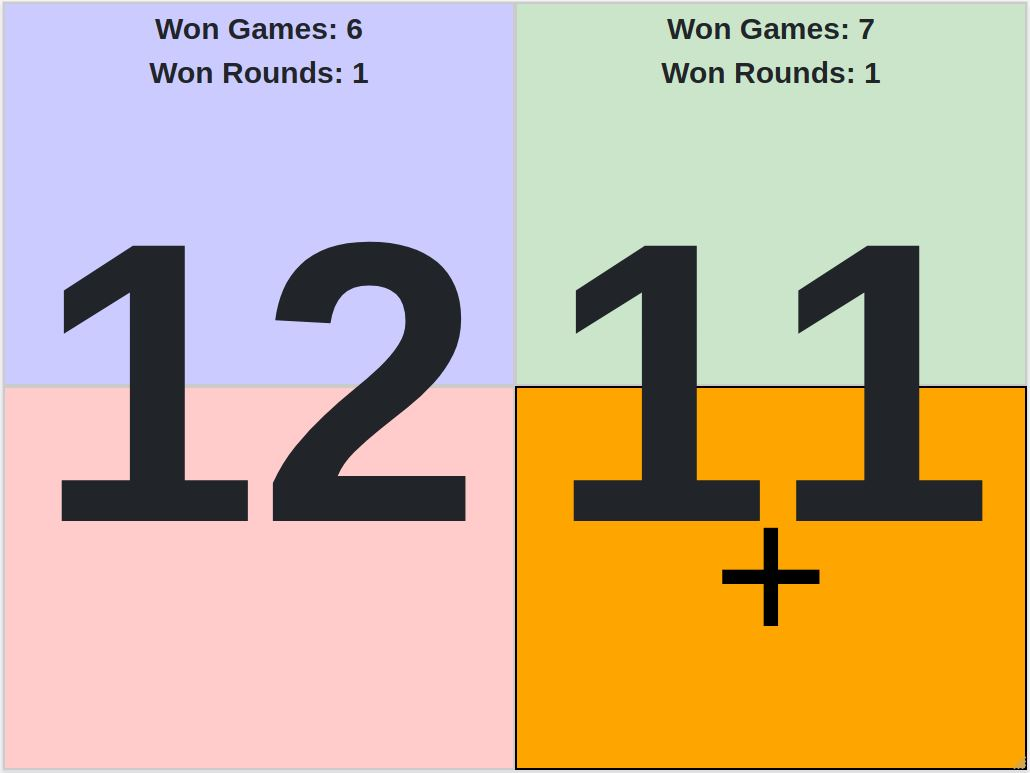
\includegraphics[scale=0.5]{Grafiken/game_seite}
\label{Game Seite}
\caption{Game-Seite der Benutzeroberfläche}
\end{figure}

In Abbildung \ref{Game Seite} ist die Game-Seite der Benutzeroberfläche dargestellt. Diese Seite stellt viele Informationen des Spiels des Benutzers dar. Die Seite ist in vier gleich große farbige Rechtecke aufgeteilt. Diese farbigen Rechtecke stellen die Position der Spieler auf dem Feld dar. Die Farben der Rechtecke entsprechen den Farben die der Benutzer für die Spieler gewählt hat. Eines der vier Rechtecke ist farbig hervorgehoben und mit einem Kreuz markiert. Dadurch wird gekennzeichnet, dass die Person, welche auf dieser Position steht, Aufschlag hat. Zusätzlich zu den Positionen der Spieler und der Aufschlaganzeige, werden die gewonnen Punkte, Sätze und Spiele des jeweiligen Teams auf der jeweiligen Seite des Spielfeldes angezeigt.
